%%%%%%%%%%%%%%%%%%%%%%%%%%%%%%%%%%%%%%%%%%%%%%%%%%%%%%%%%%%%%%%%%%%%%%%%%%%%%%%%
\chapter{РАЗРАБОТКА АЛГОРИТМА ИЗВЛЕЧЕНИЯ КОНТРАКТОВ ИЗ ИСХОДНОГО КОДА}
\label{chapter:algoritm}
%%%%%%%%%%%%%%%%%%%%%%%%%%%%%%%%%%%%%%%%%%%%%%%%%%%%%%%%%%%%%%%%%%%%%%%%%%%%%%%%
В соответствии с поставленной задачей, необходимо разработать технологию автоматического извлечения контрактов функций из исходного кода программ. Технология состоит из трех основных элементов:
\begin{itemize}
\item анализ исходного кода программы и выявление предварительных версий контрактов;
\item хранение полученной информации;
\item получение окончательных версий контрактов для функций из извлеченной информации;
\end{itemize}

Этот раздел посвящен разработке перечисленных компонентов. В разделе изложены основные идеи, положенные в их основу.

%%%%%%%%%%%%%%%%%%%%%%%%%%%%%%%%%%%%%%%%%%%%%%%%%%%%%%%%%%%%%%%%%%%%%%%%%%%%%%%%
\section{Общая схема алгоритма автоматического извлечения контрактов}
%%%%%%%%%%%%%%%%%%%%%%%%%%%%%%%%%%%%%%%%%%%%%%%%%%%%%%%%%%%%%%%%%%%%%%%%%%%%%%%%
Предлагаемая схема извлечения контрактов из исходного кода в общем виде может быть представлена следующим образом(см. рисунок \ref{image:general_scheme}). На схеме приведен алгоритм извлечения контрактов для одной функции.
\begin{figure}[h!]
\center{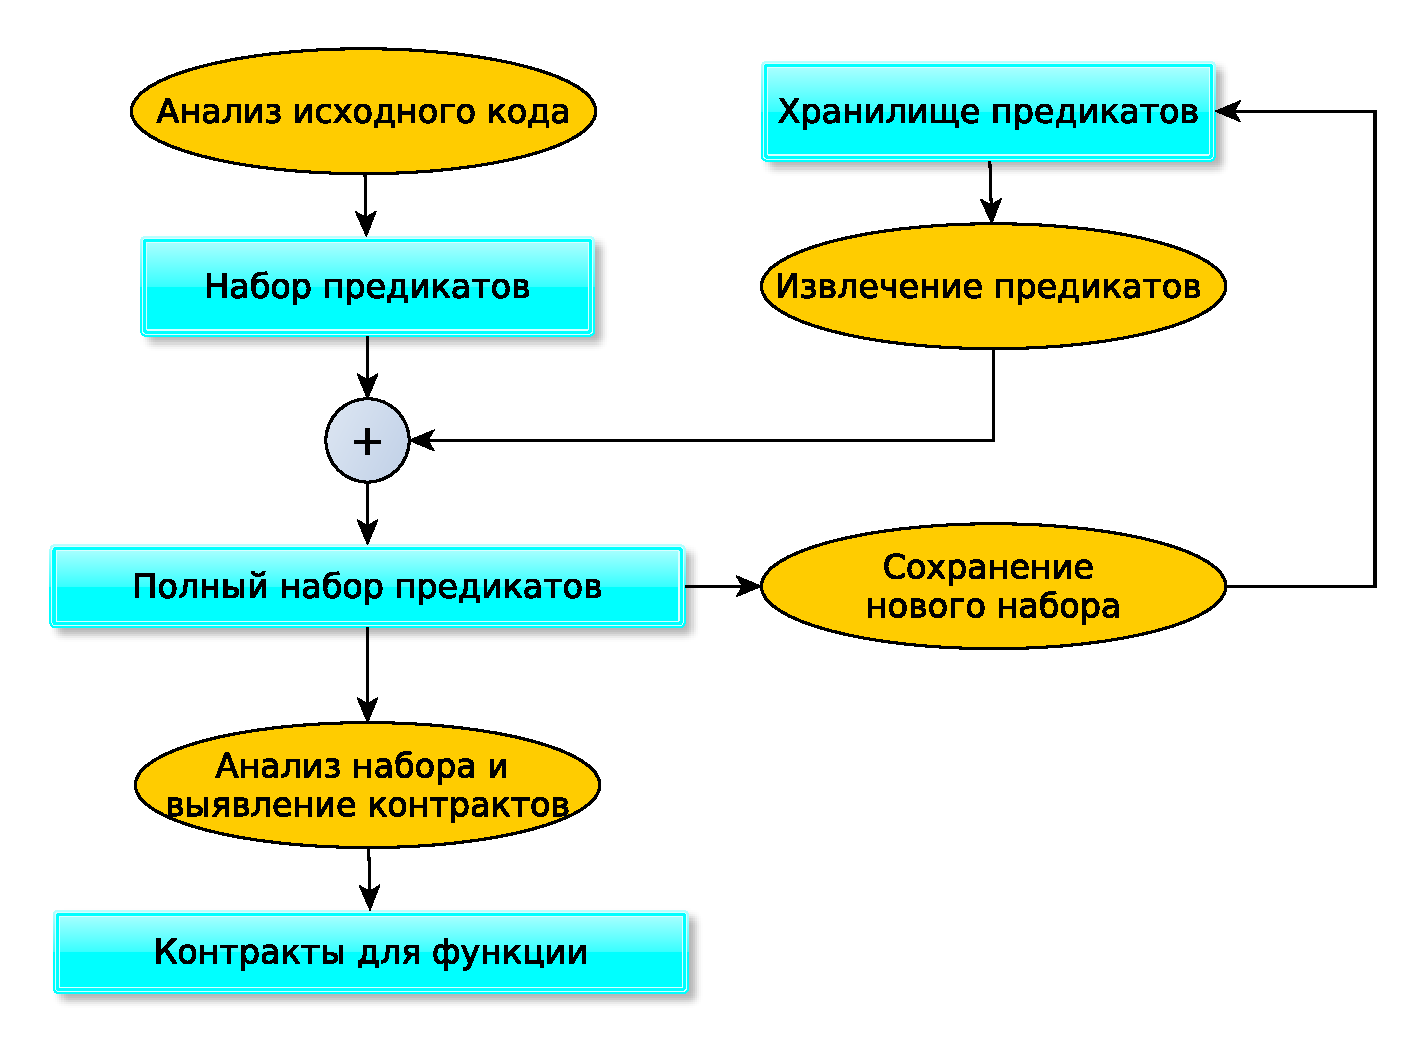
\includegraphics[width=\linewidth]{general_scheme}}
\caption{Общая схема технологии извлечения контрактов для функции из исходного кода}
\label{image:general_scheme}
\end{figure}

Алгоритм принимает на вход исходный код программы. На выходе --- сформированные контракты для функций, используемых в поданной программе. Для повышения эффективности работы алгоритма в нем так же используется хранилище предикатов. При выполнении анализа из него извлекается дополнительная информация о функции.

Главным показателем эффективности алгоритма является точность анализа, то есть вероятность извлечения некорректного контракта для функции должна быть минимальной. Остальные параметры (точность, эффективность) в данной работе считаются второстепенными.

Рассмотрим основные компоненты методики отдельно.

%%%%%%%%%%%%%%%%%%%%%%%%%%%%%%%%%%%%%%%%%%%%%%%%%%%%%%%%%%%%%%%%%%%%%%%%%%%%%%%%
\section{Извлечение предварительных версий контрактов из исходного кода}
%%%%%%%%%%%%%%%%%%%%%%%%%%%%%%%%%%%%%%%%%%%%%%%%%%%%%%%%%%%%%%%%%%%%%%%%%%%%%%%%